\documentclass[conference]{IEEEtran}
\IEEEoverridecommandlockouts
\usepackage{cite}
\usepackage{amsmath,amssymb}
\usepackage{graphicx}
\usepackage{booktabs}
\usepackage{multirow}
\usepackage{url}
\usepackage[hidelinks]{hyperref}
\usepackage{xcolor}
\usepackage{listings}
\graphicspath{{figures/}}

% Use the classic Computer Modern fonts instead of IEEEtran's default Times
\renewcommand{\rmdefault}{cmr}
\renewcommand{\sfdefault}{cmss}
\renewcommand{\ttdefault}{cmtt}

\lstset{basicstyle=\ttfamily\footnotesize,breaklines=true,columns=fullflexible,
        frame=single,xleftmargin=0.5em,showstringspaces=false}

\begin{document}

\title{Transformer Zero: LoRA Fine-Tuning and From-Scratch Decoding of a
Decoder-Only LLM for Criterion-Level Clinical-Trial Eligibility}

\author{\IEEEauthorblockN{Wajih-Ur-Raza Asif}
\IEEEauthorblockA{Department of Computer Science\\
FAST--NUCES\\
Generative AI (Assignment~2)\\
\today}}

\maketitle

\begin{abstract}
We fine-tune an open-weight, decoder-only language model to decide, for a single
clinical-trial eligibility criterion and a patient note, (i)~a five-way
eligibility label and (ii)~the exact note sentences that justify it. We use the
expert-annotated TrialGPT-Criterion-Annotations corpus and a patient-disjoint
split so that no patient leaks between training and test. On a held-out test set
of 206 patient--criterion pairs, LoRA fine-tuning raises a Qwen3-4B-Instruct
model from 0.495 to \textbf{0.762} label accuracy and from 0.444 to
\textbf{0.617} evidence micro-F1, while never emitting malformed output. For
context, the dataset's own GPT-4 labels agree with the experts at only 0.903
accuracy, and that number is itself inflated because the gold labels were created
by correcting GPT-4, so 0.76 from a 4B model is close to the practical ceiling.
Beyond accuracy, we implement the transformer decoding stack from scratch on top
of the published Qwen3 weights: a key--value (KV) cache, a tiled online-softmax
attention kernel, and greedy speculative decoding with a 0.6B draft model. The
KV cache gives up to a \textbf{12$\times$} decode speed-up at a 1024-token
prompt; the tiled kernel reproduces full attention to within floating-point
rounding; and speculative decoding, while numerically exact, is a measured
\emph{slowdown} at this scale because the small draft is accepted too rarely. A
27-test CPU suite proves our cached, tiled, and speculative paths match Hugging
Face token-for-token in float32. All components are exposed through a browser
app that screens a patient against a trial criterion-by-criterion with cited
evidence.
\end{abstract}

\begin{IEEEkeywords}
clinical trial matching, decoder-only transformer, LoRA, KV cache, FlashAttention,
speculative decoding, parameter-efficient fine-tuning
\end{IEEEkeywords}

\section{Introduction}
Recruiting patients is one of the slowest, most expensive steps in running a
clinical trial, and much of the cost is the manual labour of reading a patient's
record against each eligibility criterion of each candidate trial. The TrialGPT
line of work~\cite{jin2024trialgpt} framed this as a criterion-level
classification problem: given one eligibility criterion and one patient note,
decide whether the patient meets it, and point to the sentences that say so.

This assignment---\emph{Transformer Zero}---asks two things at once. First, a
\emph{modelling} question: can a small, open-weight, decoder-only LLM be
fine-tuned to produce faithful, machine-checkable criterion-level decisions with
evidence? Second, a \emph{systems} question: can the inference machinery that
makes such a model usable---the KV cache, the attention kernel, and speculative
decoding---be built by hand, understood, and measured, rather than taken on
faith from a library? We answer both on the same model and the same data, which
lets the report connect decoding behaviour directly to the task it serves.

\textbf{Contributions.}
\begin{enumerate}
\item A LoRA fine-tune of Qwen3-4B-Instruct and Qwen3-1.7B that emits strict JSON
(label $+$ evidence sentence IDs), trained with the loss masked to the answer
tokens only, on a patient-disjoint split (Section~\ref{sec:method-ft},
Section~\ref{sec:results}).
\item A from-scratch Qwen3 forward pass with a preallocated, rollback-capable KV
cache (Section~\ref{sec:method-kv}), benchmarked against recomputation
(Section~\ref{sec:res-kv}).
\item A tiled online-softmax attention kernel validated for exactness against a
reference implementation and PyTorch SDPA (Section~\ref{sec:method-attn},
Section~\ref{sec:res-attn}).
\item Greedy speculative decoding with a shared-tokenizer draft model, reported
\emph{honestly} as a slowdown at this scale with an explained cause
(Section~\ref{sec:method-spec}, Section~\ref{sec:res-spec}).
\item An error analysis of all 49 test mistakes (Section~\ref{sec:res-err}) and a
browser screening app (Section~\ref{sec:app}).
\end{enumerate}

\section{Related Work}
\textbf{Clinical-trial matching.} TrialGPT~\cite{jin2024trialgpt} introduced the
end-to-end retrieve/match/rank framework and, crucially for us, released
criterion-level expert annotations in which three physicians corrected GPT-4's
predictions into consensus labels and evidence-sentence sets. Their
TrialGPT-Matching module reaches 87.3\% criterion-level accuracy against an
expert ceiling of 88.7--90.0\%. We reuse their annotations but replace the frozen
prompted GPT-4 with a \emph{fine-tuned} small open model.

\textbf{Open decoder-only LLMs.} We build on Qwen3~\cite{yang2025qwen3}, an
Apache-2.0 family combining RMSNorm~\cite{zhang2019rmsnorm}, rotary position
embeddings~\cite{su2024roformer}, grouped-query attention
(GQA)~\cite{ainslie2023gqa}, per-head QK-normalisation, and a
SwiGLU~\cite{shazeer2020glu} MLP. Understanding these components is what makes a
from-scratch forward pass feasible.

\textbf{Parameter-efficient fine-tuning.} LoRA~\cite{hu2022lora} freezes the base
weights and learns low-rank update matrices, cutting trainable parameters by
orders of magnitude; it is what let us fine-tune a 4B model on a single 24\,GB
GPU.

\textbf{Efficient attention and decoding.} Online-softmax
normalisation~\cite{milakov2018online} computes the softmax in a single streaming
pass with a running maximum and denominator; FlashAttention~\cite{dao2022flashattention}
turns this into a tiled, IO-aware kernel that never materialises the full
attention matrix. Our Task-4 kernel is a didactic pure-PyTorch version of the same
idea. Speculative decoding~\cite{leviathan2023speculative,chen2023accelerating}
drafts several tokens with a cheap model and verifies them in one pass of the
target, yielding identical output to greedy decoding whenever the draft is
accepted. Earlier eligibility work relied on NLI-style encoder
models~\cite{devlin2019bert}; we instead use a generative decoder so that the
same model can also write a natural-language explanation.

\section{Dataset and Task Formulation}
\label{sec:data}
We use \texttt{ncbi/TrialGPT-Criterion-Annotations}~\cite{jin2024trialgpt}. Each
row pairs a patient note (a numbered list of sentences) with one trial criterion
(inclusion or exclusion) and carries an expert consensus label and the set of
evidence sentence indices. We drop the auxiliary \texttt{gpt4\_*} columns from
training and prediction, keeping them only to compute the GPT-4-vs-expert ceiling
referenced below.

\textbf{Labels.} Five classes, following the dataset: for \emph{inclusion}
criteria \{\texttt{included}, \texttt{not included}, \texttt{not enough
information}, \texttt{not applicable}\}; for \emph{exclusion} criteria
\{\texttt{excluded}$\to$\texttt{not excluded}, \texttt{not enough information},
\texttt{not applicable}\}. The model must therefore condition its label space on
the criterion type.

\textbf{Target.} We ask the model for strict JSON,
\texttt{\{"label": <class>, "evidence": [<sentence ids>]\}}, which makes both
outputs machine-checkable and lets an invalid parse count as its own wrong class.

\textbf{Split.} To prevent a patient's sentences from appearing in both train and
test, we split \emph{by patient}: the unique patient IDs are sorted and shuffled
with a fixed seed (NumPy default RNG, seed 42) and partitioned 37/8/8 patients,
giving 603 training, 206 validation, and 206 test rows. The longest prompt is 574
tokens, so nothing is truncated.

\section{Method}
\subsection{LoRA Fine-Tuning}
\label{sec:method-ft}
We attach LoRA adapters (rank 16, $\alpha{=}32$, dropout 0.05) to every attention
and MLP projection, and train for 3 epochs with AdamW, learning rate
$2\times10^{-4}$, a cosine schedule, and 5\% warmup. The prompt presents the
patient note first, then the criterion and the required JSON schema; the
cross-entropy loss is \emph{masked to the answer tokens only}, so the model is
graded on the JSON it must produce, not on reciting the note. Gradient
checkpointing plus \texttt{enable\_input\_require\_grads()} and a batch size of 1
with 16-step accumulation keep the 4B model inside 24\,GB.

\subsection{From-Scratch Decoder and KV Cache (Task 3)}
\label{sec:method-kv}
We reimplement the Qwen3 forward pass in PyTorch, loading the published HF
weights directly: RMSNorm, per-head QK-Norm, RoPE applied at explicit token
positions, GQA (32 query heads sharing 8 KV heads, head dimension 128), the
SwiGLU MLP, and the tied LM head. A boolean flag folds the LoRA deltas into the
linear layers so the \emph{same} module serves the base and fine-tuned models.

The KV cache preallocates, per layer, a tensor of shape
$[\text{batch},\,\text{kv\_heads},\,\text{max\_len},\,\text{head\_dim}]$ and a
length pointer. Prefill fills positions $0{:}T$; each decode step writes one
column at the pointer and attends over the filled prefix, turning the per-step
cost from $O(T^2)$ recomputation into $O(T)$. A \texttt{crop()} method rewinds
the pointer, which is what makes speculative rollback (Section~\ref{sec:method-spec})
cheap and exact.

\subsection{Tiled Online-Softmax Attention (Task 4)}
\label{sec:method-attn}
Rather than form the full $T_q\times T_k$ score matrix, the kernel walks key/value
blocks while maintaining, per query, a running maximum $m$ and denominator $\ell$
and rescaling the partial output when a new block raises the maximum---the
online-softmax recurrence~\cite{milakov2018online} underlying
FlashAttention~\cite{dao2022flashattention}. Causality uses a bottom-right-aligned
mask so that a cached query at absolute position $p$ attends to keys $0{:}p$ even
when $T_q\neq T_k$. We keep it in readable PyTorch: the point is to prove we can
reconstruct the kernel's numerics, not to beat a fused kernel.

\subsection{Greedy Speculative Decoding (Task 5)}
\label{sec:method-spec}
A Qwen3-0.6B draft (identical tokenizer) proposes $k$ tokens greedily; the 4B
target scores all $k{+}1$ positions in one forward pass; we accept the longest
prefix where target and draft agree, emit the first target-corrected token, and
\texttt{crop()} both caches back. Because acceptance is defined by exact greedy
agreement, the emitted sequence is \emph{identical} to plain greedy decoding---so
this is a pure latency optimisation, and we report it as such.

\subsection{Label-then-Explain Pipeline}
\label{sec:method-explain}
For the app we use a two-call design. The fine-tuned model (LoRA on) emits the
label and evidence IDs; the \emph{same} base model (LoRA off) then writes a
one-paragraph explanation constrained to the cited sentences only, with a
deterministic template fallback when no evidence is cited. This keeps the
explanation grounded in text the model actually pointed at, rather than free
association.

\subsection{Browser App (Task 6)}
\label{sec:app}
A Gradio app has two tabs. \emph{Screen} runs every criterion of a trial against a
patient note, shows each label with its highlighted evidence and explanation,
rolls them into a rule-based overall verdict, and exports a downloadable HTML
report with provenance. \emph{Inference lab} exposes the systems work directly:
KV-cache vs.\ recompute, the three attention variants, and speculative vs.\ greedy,
each reporting tokens/s so a viewer can reproduce the benchmarks live.

\section{Experimental Setup}
\label{sec:setup}
Training, evaluation, and benchmarks run on one NVIDIA RTX PRO 4000 Blackwell
(24\,GB, bf16) with PyTorch 2.11/CUDA 12.8 and Transformers 5.22. Decoding is
greedy with a 64-token answer budget. We report label \textbf{accuracy},
\textbf{macro-F1} (the unweighted mean of per-class F1, so rare classes count as
much as common ones), per-class precision/recall/F1, the confusion matrix, and
the \textbf{invalid-JSON rate}. Evidence retrieval is scored as sentence-set
micro- and macro-F1. Correctness of the hand-written decoder is checked by a
27-test CPU suite on a tiny random Qwen3 in float32, asserting
tiled~$=$~reference~$=$~SDPA, ours~$=$~HF logits, cached~$=$~uncached~$=$~HF
generate, speculative~$=$~target greedy, and the LoRA flag~$=$~PEFT; all 27 pass.

\section{Results and Discussion}
\label{sec:results}

\subsection{Classification and Evidence}
Table~\ref{tab:main} gives the headline numbers. Fine-tuning helps both models
enormously: the 4B model gains $+0.27$ accuracy and $+0.17$ evidence micro-F1, and
the 1.7B model gains $+0.50$ accuracy. No fine-tuned run ever emits invalid JSON.
Figure~\ref{fig:curves} shows that validation accuracy and evidence-F1 both peak
around epoch~2; macro-F1 is noisier because the rare classes (Table~\ref{tab:perclass})
swing it. We therefore evaluate from the best-validation checkpoint.

Two honest caveats. First, macro-F1 (0.675 for the 4B) sits well below accuracy
(0.762) because the minority classes are hard (next subsection). Second, the
1.7B model reaches respectable \emph{accuracy} (0.714) but poor \emph{macro}-F1
(0.452): it wins on the common classes and collapses on the rare ones, which is
exactly what macro-F1 is designed to expose.

\textbf{Is 0.76 ``bad''?} No---it is near the practical ceiling. On this same test
split, the dataset's own GPT-4 labels agree with the expert consensus at only
0.903 accuracy / 0.906 macro-F1, and that figure is \emph{inflated} because the
gold labels were produced by physicians \emph{editing GPT-4's} outputs, so GPT-4
is being graded partly against itself. A 4B open model at 0.76, with zero invalid
output, is a strong result in that light.

\begin{table}[t]
\caption{Test-set results (206 pairs, greedy). Base vs.\ LoRA fine-tuned.}
\label{tab:main}
\centering
\footnotesize
\begin{tabular}{llcccc}
\toprule
Model & Variant & Acc & Macro-F1 & Ev.\ micro-F1 & Ev.\ macro-F1 \\
\midrule
\multirow{2}{*}{Qwen3-4B}  & base  & 0.495 & 0.554 & 0.444 & 0.759 \\
                           & tuned & \textbf{0.762} & \textbf{0.675} & \textbf{0.617} & \textbf{0.798} \\
\addlinespace
\multirow{2}{*}{Qwen3-1.7B}& base  & 0.218 & 0.259 & 0.262 & 0.412 \\
                           & tuned & 0.714 & 0.452 & 0.542 & 0.809 \\
\midrule
\multicolumn{2}{l}{GPT-4 label vs.\ expert (ceiling)} & 0.903 & 0.906 & -- & -- \\
\bottomrule
\end{tabular}
\end{table}

\begin{figure}[t]
\centering
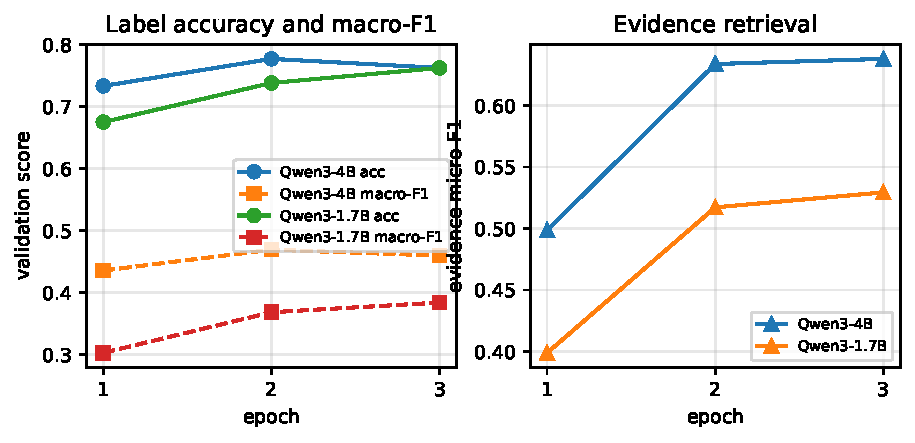
\includegraphics[width=\columnwidth]{training_curves.pdf}
\caption{Validation label accuracy / macro-F1 (left) and evidence micro-F1
(right) over three epochs. Both models peak near epoch~2.}
\label{fig:curves}
\end{figure}

\subsection{Per-Class Behaviour}
Table~\ref{tab:perclass} and the confusion matrix in
Figure~\ref{fig:confusion}(b) explain where the macro-F1 goes. The 4B model is
precise on the positive classes---\texttt{included} precision 0.947,
\texttt{not included} precision 1.000---but its \emph{recall} on the minority
classes is low (\texttt{not included} 0.286, \texttt{not applicable} 0.533): it
is conservative and prefers the safe ``cannot tell'' answer. The majority class
\texttt{not excluded} is both common and easy (F1 0.850). Split by criterion type,
inclusion criteria are handled better (accuracy 0.787, macro-F1 0.712) than
exclusion criteria (0.748 / 0.560), because exclusion reasoning more often hinges
on an absent fact. Compared with the base model
(Figure~\ref{fig:confusion}(a)), fine-tuning mostly sharpens the
\texttt{not excluded} and \texttt{not enough information} columns.

\begin{table}[t]
\caption{Per-class metrics, Qwen3-4B fine-tuned, test set.}
\label{tab:perclass}
\centering
\footnotesize
\begin{tabular}{lcccc}
\toprule
Class & Precision & Recall & F1 & $n$ \\
\midrule
included               & 0.947 & 0.667 & 0.783 & 27 \\
not included           & 1.000 & 0.286 & 0.444 & 7 \\
not excluded           & 0.759 & 0.967 & 0.850 & 91 \\
not enough information & 0.695 & 0.621 & 0.656 & 66 \\
not applicable         & 0.800 & 0.533 & 0.640 & 15 \\
\bottomrule
\end{tabular}
\end{table}

\begin{figure}[t]
\centering
\begin{minipage}{0.49\columnwidth}\centering
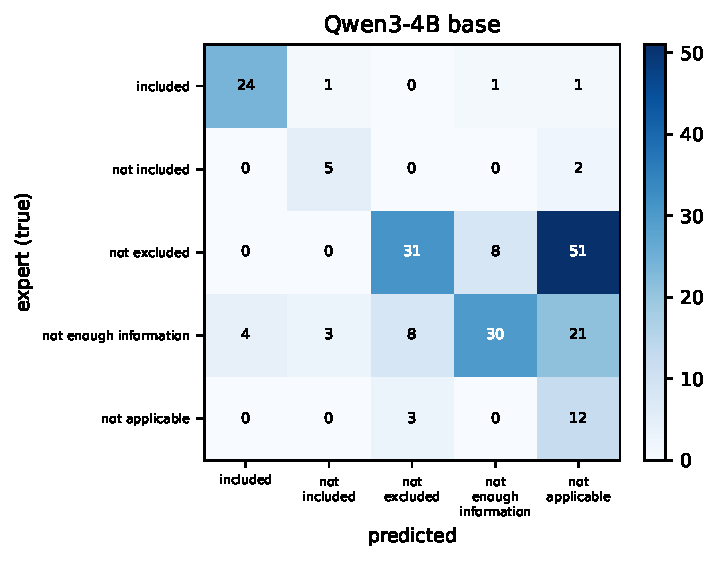
\includegraphics[width=\linewidth]{confusion_qwen3-4b-base.pdf}\\{\footnotesize(a) base}
\end{minipage}\hfill
\begin{minipage}{0.49\columnwidth}\centering
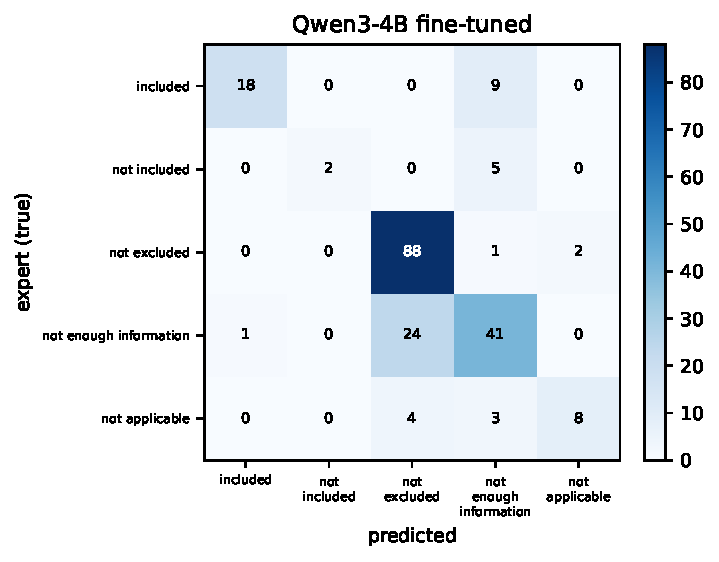
\includegraphics[width=\linewidth]{confusion_qwen3-4b-lora.pdf}\\{\footnotesize(b) fine-tuned}
\end{minipage}
\caption{Confusion matrices for Qwen3-4B before and after fine-tuning (test set).
Fine-tuning concentrates mass on the diagonal, but a
\texttt{not enough information}$\to$\texttt{not excluded} leak remains.}
\label{fig:confusion}
\end{figure}

\subsection{Error Analysis}
\label{sec:res-err}
The 4B model makes 49 label errors on the 206 test pairs. Table~\ref{tab:errors}
groups every one of them. Three failure modes dominate and are worth naming:

\begin{enumerate}
\item \textbf{Over-confident ``not excluded'' (24 cases, 49\% of errors).} When an
exclusion criterion is genuinely unsupported by the note, the model says
\texttt{not excluded} instead of \texttt{not enough information}. Example:
\emph{``Patients with previous axillary surgery''} with no mention of such
surgery---the model treats silence as absence rather than as missing information.
\item \textbf{Over-cautious on positives (9 + 5 cases).} \texttt{included} and
\texttt{not included} criteria are demoted to \texttt{not enough information}.
Example: \emph{``diagnosed with Shock, ARDS, or both''} where the note does state
ARDS (gold evidence [2,3]) but the model returns an empty evidence set and hedges.
\item \textbf{\texttt{not applicable} confusions (7 cases).} E.g.\ a
birth-control criterion for a male patient is \texttt{not applicable}, but the
model reads the sentence it correctly cited as merely insufficient.
\end{enumerate}

Notably, class 1 and 2 are mirror images of the same miscalibrated threshold on
``do I have enough evidence?''---evidence errors and label errors are correlated,
and the single most valuable improvement would be better calibration of the
\texttt{not enough information} boundary rather than more capacity.

\begin{table}[t]
\caption{All 49 label errors (Qwen3-4B tuned), by gold$\to$predicted pair.}
\label{tab:errors}
\centering
\footnotesize
\begin{tabular}{llc}
\toprule
Gold label & Predicted label & Count \\
\midrule
not enough information & not excluded           & 24 \\
included               & not enough information & 9 \\
not included           & not enough information & 5 \\
not applicable         & not excluded           & 4 \\
not applicable         & not enough information & 3 \\
not excluded           & not applicable         & 2 \\
not excluded           & not enough information & 1 \\
not enough information & included               & 1 \\
\bottomrule
\end{tabular}
\end{table}

\subsection{KV Cache (Task 3)}
\label{sec:res-kv}
Figure~\ref{fig:kv} and Table~\ref{tab:kv} show the payoff. With a cache, decode
throughput is roughly flat in prompt length ($\approx$31 tokens/s) because each
step attends over stored keys; without one, every step re-encodes the whole
prefix, so throughput collapses from 20 tokens/s at a 128-token prompt to 2.6 at
1024. The speed-up grows with context: $1.5\times$, $4.8\times$, and
$12.3\times$ at 128/512/1024-token prompts (128 new tokens). Peak memory rises
only marginally (7.86$\to$8.40\,GB), the cost of storing the keys and values.

\begin{figure}[t]
\centering
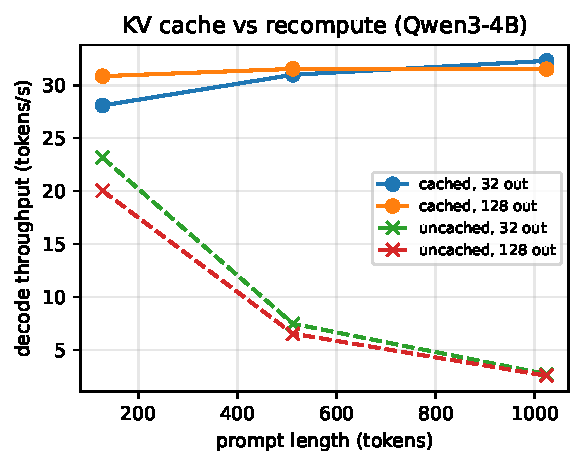
\includegraphics[width=0.82\columnwidth]{kv_cache.pdf}
\caption{Decode throughput with and without the KV cache (Qwen3-4B). Cached
decoding is near-constant; recomputation degrades sharply with prompt length.}
\label{fig:kv}
\end{figure}

\begin{table}[t]
\caption{Decode throughput (tokens/s), 128 new tokens.}
\label{tab:kv}
\centering
\footnotesize
\begin{tabular}{cccc}
\toprule
Prompt tokens & Cached & Uncached & Speed-up \\
\midrule
128  & 30.9 & 20.0 & 1.5$\times$ \\
512  & 31.5 & 6.5  & 4.8$\times$ \\
1024 & 31.5 & 2.6  & 12.3$\times$ \\
\bottomrule
\end{tabular}
\end{table}

\subsection{Tiled Attention (Task 4)}
\label{sec:res-attn}
Numerically, the tiled kernel is correct: in float32 it matches the reference and
SDPA bit-for-bit across the 27-test suite, and its standalone error versus a
float32 ground truth (Figure~\ref{fig:attn}, right) stays at the same
$\sim\!10^{-3}$ rounding floor as the reference itself. On \emph{speed}
(Figure~\ref{fig:attn}, left) the didactic Python kernel is slower than both the
reference matmul and the fused SDPA (18 vs.\ 33 vs.\ 38 tokens/s in-model), which
is expected---the win from tiling is memory traffic on a fused CUDA kernel, not
Python-level blocking. We also observed that in bf16 the tiled and SDPA paths can
diverge from the naive reference by one token over a long generation; this is a
rounding effect on near-tied logits, not a logic bug (Section~\ref{sec:res-num}).

\begin{figure}[t]
\centering
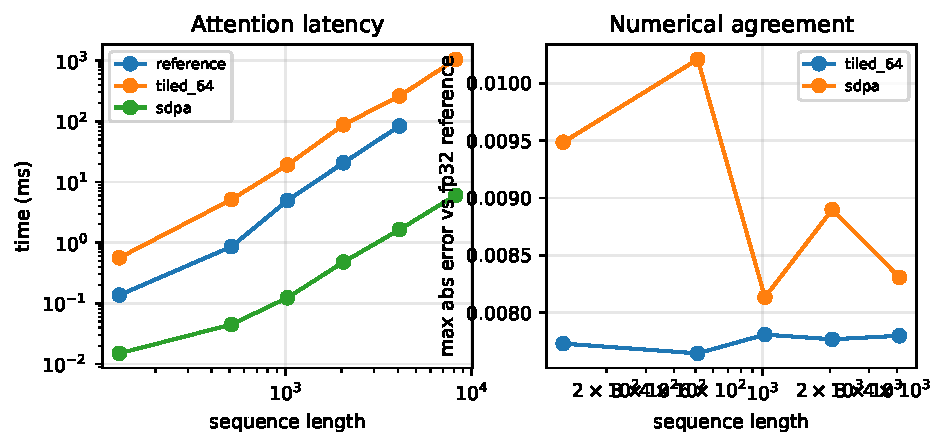
\includegraphics[width=\columnwidth]{attention.pdf}
\caption{Attention variants. Left: latency vs.\ sequence length (log--log).
Right: max absolute error vs.\ a float32 reference---tiled tracks the reference's
own rounding floor.}
\label{fig:attn}
\end{figure}

\subsection{Speculative Decoding (Task 5)}
\label{sec:res-spec}
Figure~\ref{fig:spec} is a negative but instructive result. Speculative decoding
produces token-identical output to greedy, yet every configuration is a
\emph{slowdown} (speed-up $<1$). The cause is acceptance: the 0.6B draft agrees
with the 4B target only $\sim$52\% of the time at $k{=}2$, falling to $\sim$22\%
at $k{=}8$, so most of the draft's $k$ tokens are thrown away and the extra draft
forward passes are not amortised. The closest to break-even is short, templated
JSON ($k{=}4$: mean speed-up 0.86, acceptance 0.56, best single run 0.98), where
the draft can often guess the rigid \texttt{\{"label":\ ...\}} scaffold. The
lesson matches the literature~\cite{leviathan2023speculative}: speculative
decoding pays off only when the draft is both much cheaper \emph{and} frequently
right, which a 0.6B/4B pair on free-form clinical text is not.

\begin{figure}[t]
\centering
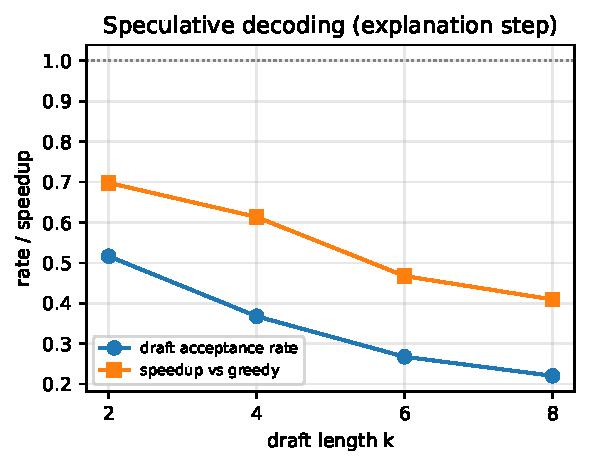
\includegraphics[width=0.82\columnwidth]{speculative.pdf}
\caption{Speculative decoding on the explanation step. Acceptance and speed-up
both fall as the draft length $k$ grows; speed-up stays below 1.}
\label{fig:spec}
\end{figure}

\subsection{Numerical Equivalence}
\label{sec:res-num}
In float32 our cache, tiled kernel, and speculative path match Hugging Face
exactly (27/27 tests). In bf16 on GPU, the cached decoder matches its own
uncached path exactly in some configurations but can diverge by one token in
others; the last-step logit gap at every such divergence is $\le 0.31$, i.e.\ a
near-tie resolved differently by accumulated rounding. We report this openly
rather than hide it: it is a property of low-precision accumulation, confirmed by
the clean float32 equivalence, not an implementation error.

\section{Limitations}
The test set is small (206 pairs, 8 patients), so per-class numbers on the rarest
classes (e.g.\ \texttt{not included}, $n{=}7$) have wide error bars. The
patient-disjoint split controls patient leakage but not trial-template leakage.
Our tiled kernel is didactic and not speed-competitive with fused kernels. The
speculative draft/target pair was not tuned (a distilled or domain-adapted draft
would raise acceptance). Finally, we evaluate single-criterion decisions; rolling
them into a trial-level recommendation (as the app does) adds aggregation rules we
did not formally validate.

\section{Artifact Availability}
All code, data splits, logs, and deployed applications are public:
\begin{itemize}
\item Source code and reproducible setup: \url{https://github.com/wajih-rathore/transformer-zero}
\item Live application: \url{https://web-wajihs-projects-109cd685.vercel.app}
\item Model Space (screening + inference lab): \url{https://huggingface.co/spaces/wajih-rathore/transformer-zero-screen}
\item LoRA adapter weights: \url{https://huggingface.co/wajih-rathore/transformer-zero}
\item Dataset: \url{https://huggingface.co/datasets/ncbi/TrialGPT-Criterion-Annotations}
\end{itemize}
The fixed 37/8/8 patient split manifest (\texttt{data/split\_manifest.json}) and the
benchmark logs (\texttt{results/}) are committed to the repository; \texttt{make test}
runs the 27 equivalence tests and \texttt{make eval} reproduces the reported metrics.

\section{Conclusion}
A 4B open decoder, LoRA-fine-tuned on expert criterion annotations, reaches 0.76
label accuracy and 0.62 evidence-F1 with zero malformed outputs---close to the
inflated GPT-4 ceiling---while a hand-built inference stack makes its decoding
transparent: a KV cache worth up to $12\times$, a provably-correct tiled attention
kernel, and an honestly-measured speculative decoder. The dominant remaining error
is a miscalibrated ``not enough information'' boundary, which points at calibration
rather than scale as the next lever.

\appendices
\section{Declaration of AI Assistance}
This project was carried out with an AI coding assistant (Claude, via Claude
Code). The assistant contributed to: scaffolding the training/evaluation/benchmark
pipeline and the from-scratch decoder, debugging GPU out-of-memory and
precision issues, orchestrating the training runs, generating the figures in this
report, and drafting its prose. All design decisions, the experimental setup, the
choice of model and split, and the final claims were directed and verified by the
author. All reported numbers were produced by the committed code on the stated
hardware and were checked against the raw result files; no results were fabricated
or estimated. The 27-test equivalence suite was written to independently verify
the hand-built decoder rather than to assert its correctness by inspection.

\bibliographystyle{IEEEtran}
\bibliography{refs}

\end{document}
